\documentclass[11pt]{article}
\hoffset -0.5in
\voffset -1in
\textheight 9in
\textwidth 6in
\pagestyle{plain}

\usepackage{graphicx}
\usepackage[mathscr]{eucal}
\usepackage{amsmath}
\usepackage{amssymb}
\usepackage{amsthm}
\usepackage{amscd}
\usepackage{verbatim}

%\usepackage{setspace}
%\onehalfspacing
%\doublespacing

\title{ELEC 241: CA Session 5 Notes}
\author{Onkur Sen}
\date{September 26, 2012}

\begin{document}
\maketitle

\section*{Node Method}

The node method is a powerful way to find specific voltage levels and currents in a circuit. Basically, a node is formed at the juncture of two circuit elements: two resistors in series, a branch into a group of parallel elements, etc. The interesting thing about nodes is that you can apply KCL and KVL to them in the following way:

\begin{itemize}
\item {\bf The net current in the node is zero}. That is, the current coming in is equal to the current coming out. You can use this particularly in branches for parallel elements (i.e., the input current is entirely distributed across the multiple elements).
\item Suppose you have two nodes $e_1$ and $e_2$ with a collection of circuit elements between them, and suppose that the equivalent impedance of this group is $Z$. Then the total current flowing between the two nodes is $\frac{e_1-e_2}{Z}$. This is useful if you know node voltages and need to find currents (as you'll see in the case of op-amps below).
\end{itemize} 

\section*{Op-Amps}
Here's a picture of a typical inverting amplifier:
\begin{center}
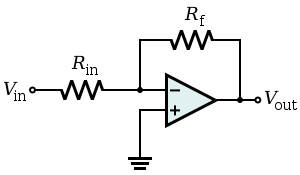
\includegraphics[scale=0.7]{opamp.png}
\end{center}
Let's take a look and notice some properties of the op-amp:
\begin{itemize}
\item {\bf No current flows through the op-amp.} In this case, that means that all of the current will go through $R_f$. (In reality, of course, {\em some} current will go through the op-amp, but it is negligible because the internal resistance of the op-amp is huge compared to anything else.)
\item $\boxed{V_+ = V_-}$, i.e., {\bf the voltage at the positive and negative terminals are the same}. This is often called the "virtual short." In this case, since the positive terminal is connected to ground, it must be the case that $V_+ = V_- = 0$.
\end{itemize}
Let's solve for $V_{out}$ in this circuit. You can find the current $i$ by using the node method at the negative terminal, i.e.:
\[i = \frac{V_{in} - V_-}{R_{in}} = \frac{V_{in}}{R_{in}} \]
We know that all of the current flows through $R_f$, so we can find $V_{out}$:
\[ V_{out} = V_- - iR_f = 0 - \frac{V_{in}}{R_{in}} R_f = \boxed{- \frac{R_f }{R_{in}} V_{in}.}\]
This is the result you derived in class.\\

\noindent A few other tips to keep in mind:
\begin{itemize}
\item If you have multiple op-amps combined with power sources, superposition is your best bet to solve the circuit.
\item In the case of the inverting amplifier, nothing was connected to the positive terminal besides ground. If you do have something else there, you can apply KVL on the positive terminal as well to get the relationships necessary to solve for $V_{out}$.
\end{itemize}

\end{document}